%%
%% YMDS AI — Main Paper
%% Target: Expert Systems with Applications (Elsevier)
%% Template: Elsevier CAS Double-Column (cas-dc)
%% Compiler: pdflatex → bibtex → pdflatex × 2
%%

\documentclass[a4paper,fleqn]{cas-dc}

%% ── Packages ────────────────────────────────────────────────────────────────
\usepackage[numbers]{natbib}
\usepackage{graphicx}
\usepackage{amsmath}
\usepackage{amssymb}
\usepackage{booktabs}
\usepackage{tabularx}
\usepackage{multirow}
\usepackage{xcolor}
\usepackage{url}
\usepackage{microtype}
\usepackage{enumitem}
\usepackage{subcaption}
\usepackage[T1]{fontenc}
\usepackage[utf8]{inputenc}
\usepackage{float}
\usepackage{placeins}
\usepackage[ruled,linesnumbered]{algorithm2e}

%% ── Running Headers ─────────────────────────────────────────────────────────
\shorttitle{YMDS AI: RAG-Based Regulatory Compliance Checking}
\shortauthors{A. Berk, U. Akgül et~al.}

%% ════════════════════════════════════════════════════════════════════════════
\begin{document}
\let\WriteBookmarks\relax
\def\floatpagepagefraction{1}
\def\textpagefraction{.001}

%% ── Title ───────────────────────────────────────────────────────────────────
\title[mode=title]{YMDS AI: A Retrieval-Augmented Generation Framework
  for Automated University Regulatory Compliance Checking}

%% ── Authors ─────────────────────────────────────────────────────────────────
\author[1]{Asya Berk}
\ead{asya.berk@bilgi.edu.tr}
\credit{Conceptualization, Methodology, Software, Writing -- Original Draft}

\author[1]{Utku Akgul}
\ead{utku.akgul@bilgi.edu.tr}
\credit{Software, Data Curation, Validation, Visualization}

\author[1]{Tugba Dalyan}
\cormark[1]
\fnmark[1]
\ead{tugba.dalyan@bilgi.edu.tr}
\credit{Supervision, Writing -- Review \& Editing, Project Administration}

\affiliation[1]{
  organization={Department of Computer Engineering, Istanbul Bilgi University},
  addressline={Kazım Karabekir Cad. No:2/13},
  city={Istanbul},
  postcode={34060},
  country={Turkey}
}

\cortext[cor1]{Corresponding author}
\fntext[fn1]{Supervisor}

%% ── Abstract ────────────────────────────────────────────────────────────────
\begin{abstract}
Universities in Turkey must comply with regulations set by the Higher Education Council
(YÖK), a process currently carried out manually by administrative staff who must read
through long, dense legal documents. We present \textbf{YMDS AI}, a
retrieval-augmented generation (RAG) system that automatically assesses whether
institutional policy documents conform to applicable YÖK regulations. The system indexes
nine official regulatory documents and evaluates five retrieval pipeline variants ---
sparse BM25, dense vector search (FAISS), a hybrid of the two, multi-query expansion,
and a no-RAG baseline --- each combined with GPT-4o and GPT-4o-mini, for ten
configurations in total. To enable meaningful evaluation, we constructed a
\textit{RAG-aware} benchmark of 40 compliance cases drawn from specific YÖK article
passages, designed so that correct answers require access to the regulatory text. Our
best configuration (Hybrid or BM25 with either model) achieves 47.5\% accuracy compared
to 37.5\% for the no-RAG baseline, a 10 percentage point improvement. GPT-4o-mini
matches GPT-4o accuracy at approximately 18$\times$ lower cost. Ablation studies
identify a chunk size of 350 words and retrieval depth of $K{=}5$ as optimal settings.
We also find that all models exhibit a systematic bias toward the \textit{partial} label
and rarely predict \textit{non-compliant}, even for clear violations --- a finding with
important practical implications for deployment. The system, benchmark dataset, and
evaluation scripts are open-sourced to support future research.
\end{abstract}

%% ── Graphical Abstract ───────────────────────────────────────────────────────
%% Uncomment when graphical abstract PDF is ready:
%% \begin{graphicalabstract}
%% \includegraphics{figures/graphical_abstract.pdf}
%% \end{graphicalabstract}

%% ── Highlights ───────────────────────────────────────────────────────────────
\begin{highlights}
\item First RAG-based compliance checking system for Turkish higher education regulations
\item Five retrieval pipelines evaluated: No-RAG, BM25, Dense, Hybrid, and Multi-Query
\item Hybrid + BM25 outperform no-RAG by 10 percentage points on a hard RAG-aware benchmark
\item GPT-4o-mini matches GPT-4o accuracy at 19$\times$ lower API cost
\item Ablation studies identify 350-word chunks and Top-5 retrieval as optimal settings
\end{highlights}

%% ── Keywords ─────────────────────────────────────────────────────────────────
\begin{keywords}
Retrieval-Augmented Generation \sep
Regulatory Compliance \sep
Higher Education \sep
Large Language Models \sep
BM25 \sep
Natural Language Processing \sep
YÖK
\end{keywords}

\maketitle

%% ════════════════════════════════════════════════════════════════════════════
%% SECTION 1 — INTRODUCTION
%% ════════════════════════════════════════════════════════════════════════════
\section{Introduction}
\label{sec:intro}
Imagine you are an administrator at a Turkish university.
A new internal policy lands on your desk. Before it can go into effect,
you need to verify that it complies with the regulations set by YÖK ---
the Higher Education Council that governs all Turkish universities.
That means reading through dozens of pages of dense legal text,
cross-referencing multiple regulation documents, and making judgment calls
about ambiguous wording. This process can take hours, and it has to be
repeated for every new policy.

Now imagine a system that does this automatically.

That is exactly what we built. \textbf{ComplianceAI} is a
retrieval-augmented generation (RAG) system that takes a university policy
document, searches a database of nine official YÖK regulatory documents for
the most relevant passages, and asks a large language model to decide
whether the policy is \textit{compliant}, \textit{partially compliant}, or
\textit{non-compliant} --- all in under two seconds.

\subsection*{Why RAG?}

A natural first question is: why not just ask GPT-4o directly?
The answer is that language models are trained on large amounts of text from
the internet, but they are not guaranteed to know the specific wording of a
particular YÖK regulation from 2024 --- especially the fine-grained numerical
thresholds and procedural rules that determine compliance.
RAG addresses this by retrieving the actual regulation text at query time
and feeding it to the model as context \citep{Sun2025, Hillebrand2024}.
This way, the model reasons about what the regulation \textit{actually says},
not what it \textit{thinks} it says.

To test whether this matters, we designed our evaluation specifically around
cases where the model would be likely to fail without retrieval.
As we show in Section~\ref{sec:results}, the results are clear:
RAG-based configurations outperform the no-RAG baseline by \textbf{10 percentage
points} on our benchmark.

\subsection*{What We Contribute}

This paper makes the following contributions:

\begin{itemize}
  \item We present \textbf{ComplianceAI}, a complete end-to-end system for
    automated regulatory compliance checking in Turkish higher education,
    including a FastAPI backend, a React dashboard, and five retrieval pipeline
    variants (no-RAG, BM25, Dense, Hybrid, and Multi-Query).

  \item We build the \textbf{first annotated benchmark dataset} for this domain:
    40 compliance assessment cases specifically designed to require access to
    YÖK regulation text, with balanced class distribution (13 compliant,
    14 partial, 13 non-compliant).

  \item We conduct a \textbf{systematic comparison} of all five pipeline variants
    with two LLM backends (GPT-4o and GPT-4o-mini), finding that Hybrid and
    BM25 retrieval consistently outperform other approaches, and that
    GPT-4o-mini matches GPT-4o accuracy at 19$\times$ lower cost.

  \item We run \textbf{ablation studies} on chunk size and retrieval depth,
    identifying 350-word chunks and Top-5 retrieval as the optimal settings
    for this task.

  \item We document an important \textbf{failure mode}: all models
    systematically under-predict the non-compliant class, defaulting to
    ``partial'' even for clear violations --- a finding that should
    inform any real-world deployment of similar systems.
\end{itemize}

The rest of this paper is structured as follows.
Section~\ref{sec:related} reviews related work.
Section~\ref{sec:architecture} describes the system.
Section~\ref{sec:methodology} explains how we built the benchmark and ran
the experiments.
Section~\ref{sec:setup} covers implementation details.
Section~\ref{sec:results} presents and discusses the results ---
the most important part, with five tables and four figures.
Section~\ref{sec:conclusion} wraps up with limitations and future directions.


%% ════════════════════════════════════════════════════════════════════════════
%% SECTION 2 — RELATED WORK
%% ════════════════════════════════════════════════════════════════════════════
\section{Related Work}
\label{sec:related}
Checking whether documents comply with regulations is a well-studied problem in natural language processing, but most of the existing work focuses on financial regulations, legal contracts, or software requirements rather than higher education policy. This section covers the areas most relevant to our work: automated compliance checking, legal document understanding, and retrieval-augmented generation.

\subsection{Automated Compliance Checking}

Early work on automated compliance checking used rule-based or keyword-matching systems that required significant manual engineering for each new regulation domain. More recently, machine learning approaches — and especially large language models — have made it possible to handle the ambiguity and variation in natural language regulations without hard-coded rules.

\citet{Sun2025} proposed a compliance checking framework specifically built on RAG, where relevant regulation passages are retrieved and provided to the model as grounding context. Their work is the closest in spirit to ours: they show that retrieval significantly improves compliance classification performance compared to a direct LLM approach. We build on this idea and extend it to the Turkish higher education domain, which has its own linguistic and structural challenges.

\citet{Abualhaija2022} tackled compliance checking from a requirements engineering perspective, using automated question answering to help analysts understand regulatory requirements across multiple documents. Their approach highlighted the importance of structured document representations and precise retrieval, which informed our choice to maintain paragraph-level chunks rather than full-document representations.

\citet{Masoudifard2024} explored graph-based retrieval for compliance checking, combining knowledge graphs with prompt engineering to improve traceability between requirements and regulations. While their approach requires richer document structure than raw text, their findings on multi-hop reasoning align with our observation that retrieving context from multiple regulation passages is often necessary for partial compliance cases.

\subsection{Legal and Regulatory Document Understanding}

Several works have addressed the broader challenge of understanding legal and regulatory text with NLP. \citet{Shinde2025} reviewed NLP methods for legal document understanding, noting that domain-specific tokenization and context-aware models are essential for handling legal language, which tends to be dense, formal, and full of cross-references. \citet{Singh2024} similarly demonstrated that standard NLP pipelines need adaptation for legal text analysis due to the specialized vocabulary.

\citet{Nithya2024} and \citet{Deshpande2024} both examined AI-driven approaches to legal automation more broadly. Both papers noted that while language models can handle many routine compliance tasks, edge cases involving ambiguous or conflicting regulations remain difficult and require human oversight. Our findings echo this: all of our models struggle with non-compliant cases, often defaulting to a more conservative \textit{partial} label.

\citet{Fazlija2024} implemented financial regulations using LLMs and observed similar classification behavior, where models tend to hedge rather than make definitive compliance judgments. Our work corroborates this finding in a different domain.

\subsection{Retrieval-Augmented Generation}

RAG systems address a fundamental limitation of language models: their knowledge is frozen at training time and may not include specific, up-to-date regulatory text \citep{Hillebrand2024}. By combining a retrieval component with a generation component, RAG allows the model to reason about documents it has never explicitly seen during training.

\citet{Hillebrand2024} demonstrated a RAG chatbot for regulatory compliance in an industrial quality assurance context, finding that hybrid retrieval — combining sparse and dense methods — improves coverage compared to either method alone. This motivated our inclusion of a hybrid pipeline in our evaluation.

\citet{Li2025} applied RAG combined with code generation for financial compliance checking, highlighting the value of structured outputs in compliance tasks. Their work reinforced our choice to prompt for JSON-structured compliance verdicts rather than free-form text.

\citet{Zadenoori2025} conducted a systematic literature review of LLMs in requirements engineering, noting that while LLMs show strong performance on textual reasoning tasks, domain grounding through retrieval remains an open challenge. Our results contribute empirical data points to this ongoing discussion.

\subsection{Positioning of This Work}

To our knowledge, ComplianceAI is the first RAG-based compliance checking system designed specifically for Turkish higher education regulations. Compared to the financial and legal compliance systems reviewed above, our domain presents unique challenges: regulatory text is in Turkish, covers a broad range of administrative topics, and involves frequent cross-references between different YÖK directives. We contribute (1) a working end-to-end RAG compliance system, (2) the first annotated benchmark dataset for this domain, and (3) a systematic comparison of five retrieval pipeline variants with two LLM backends.


%% ════════════════════════════════════════════════════════════════════════════
%% SECTION 3 — SYSTEM ARCHITECTURE
%% ════════════════════════════════════════════════════════════════════════════
\section{System Architecture}
\label{sec:architecture}
ComplianceAI is built as a three-layer system: a document processing layer
that builds and maintains the regulatory knowledge base, an inference backend
that handles retrieval and LLM-based reasoning, and a web interface that lets
users submit documents and read compliance reports.
Figure~\ref{fig:architecture} provides an overview of the full pipeline.

\subsection{Knowledge Base Layer}

The knowledge base consists of nine official YÖK regulatory documents,
covering topics from graduate admission requirements to financial aid rules
and international student procedures.
These documents were collected as PDFs from the YÖK website
(\url{https://www.yok.gov.tr}) and from Istanbul Bilgi University's
official resources.

\paragraph{Current approach --- manual PDF management.}
At this stage, the regulatory documents are maintained manually: when YÖK
publishes an update, the corresponding PDF is replaced in the local
document store and the indexes are rebuilt.
This works well for a prototype but is not ideal for production.

\paragraph{Future direction --- live API integration.}
YÖK publishes regulations through its official web portal, and future
versions of ComplianceAI could automate document updates by periodically
fetching new or revised regulations directly from the source.
This would eliminate the manual maintenance step and ensure the system
always reflects the current regulatory landscape --- particularly important
as YÖK regulations are updated several times per year.

Each document is split into overlapping text chunks using a sliding window:
350 words per chunk with a 59-word overlap.
The resulting corpus contains 248 chunks across nine source documents.
Two index structures are built from these chunks.
For sparse retrieval, we build a BM25 index using \texttt{rank\_bm25}.
For dense retrieval, we encode each chunk with OpenAI's
\texttt{text-embedding-3-small} model (projected to 384 dimensions)
and store the vectors in a FAISS flat inner-product index.
Both indexes are persisted to disk so they do not need to be rebuilt
on each request.

\subsection{Inference Backend}

The inference backend is implemented as a FastAPI application.
When a user submits a document and a compliance question, the backend
routes the request to one of five retrieval pipelines:

\begin{itemize}
  \item \textbf{No-RAG}: The document and question go directly to the LLM
    without any retrieved context. This is the baseline.
  \item \textbf{BM25 (Sparse)}: The query is scored against the BM25 index
    and the top-$K$ chunks are retrieved.
  \item \textbf{Dense}: The query is embedded and compared against the FAISS
    index. The top-$K$ most similar chunks are retrieved.
  \item \textbf{Hybrid}: BM25 and Dense are run independently.
    Results are merged using reciprocal rank fusion (equal 0.5/0.5 weighting)
    and the top-$K$ are kept.
  \item \textbf{Multi-Query}: The original query is expanded into three
    related sub-queries via a lightweight LLM call.
    Each sub-query is run through BM25 and results are merged.
\end{itemize}

The retrieved chunks are formatted into a structured prompt and sent to
GPT-4o or GPT-4o-mini via the OpenAI API.
The system prompt instructs the model to respond only with a JSON object
containing four fields: \texttt{compliance\_score} (0--100),
\texttt{label} (compliant / partial / non-compliant),
\texttt{explanation} (a plain-language Turkish summary), and
\texttt{articles} (a list of specific YÖK articles referenced).
Label thresholds: compliant $\geq 70$, partial $30$--$69$,
non-compliant $< 30$.
The full system prompt is listed in Appendix~\ref{app:prompt}.

\subsection{Web Interface}

\textit{[This section will be updated with final implementation details
once the frontend and backend deployment are complete.
The current prototype includes a React-based dashboard and a FastAPI
REST API. Screenshots and endpoint documentation will be added here.]}

The interface is designed to be usable by non-technical administrative staff.
Users can upload a policy document, enter a compliance question, select the
retrieval pipeline, and receive a structured compliance report in seconds.
Results are displayed with a color-coded compliance score gauge, a
plain-language explanation, and the specific YÖK articles that were
retrieved and used in the assessment.

\subsection{Generalizability}

Although ComplianceAI was built and evaluated using Istanbul Bilgi University
documents and YÖK regulations, the system architecture is not institution-specific.
Any Turkish university could use the same system by loading their own
institutional documents and the same YÖK regulatory knowledge base.
Beyond Turkey, the same RAG-based approach could be adapted for compliance
checking in other higher education regulatory systems --- for example,
ECTS regulations in Europe or ABET accreditation requirements in the US ---
by simply replacing the regulatory document collection.
The benchmark construction methodology we describe in Section~\ref{sec:methodology}
could also be reused to evaluate compliance systems in other domains.


%% Architecture figure — generated by generate_paper_figures.py + TikZ
%% Placeholder: replace with actual figure when available
\begin{figure*}[h]
  \centering
  %% Replace the fbox below with the final architecture figure before submission:
  %% 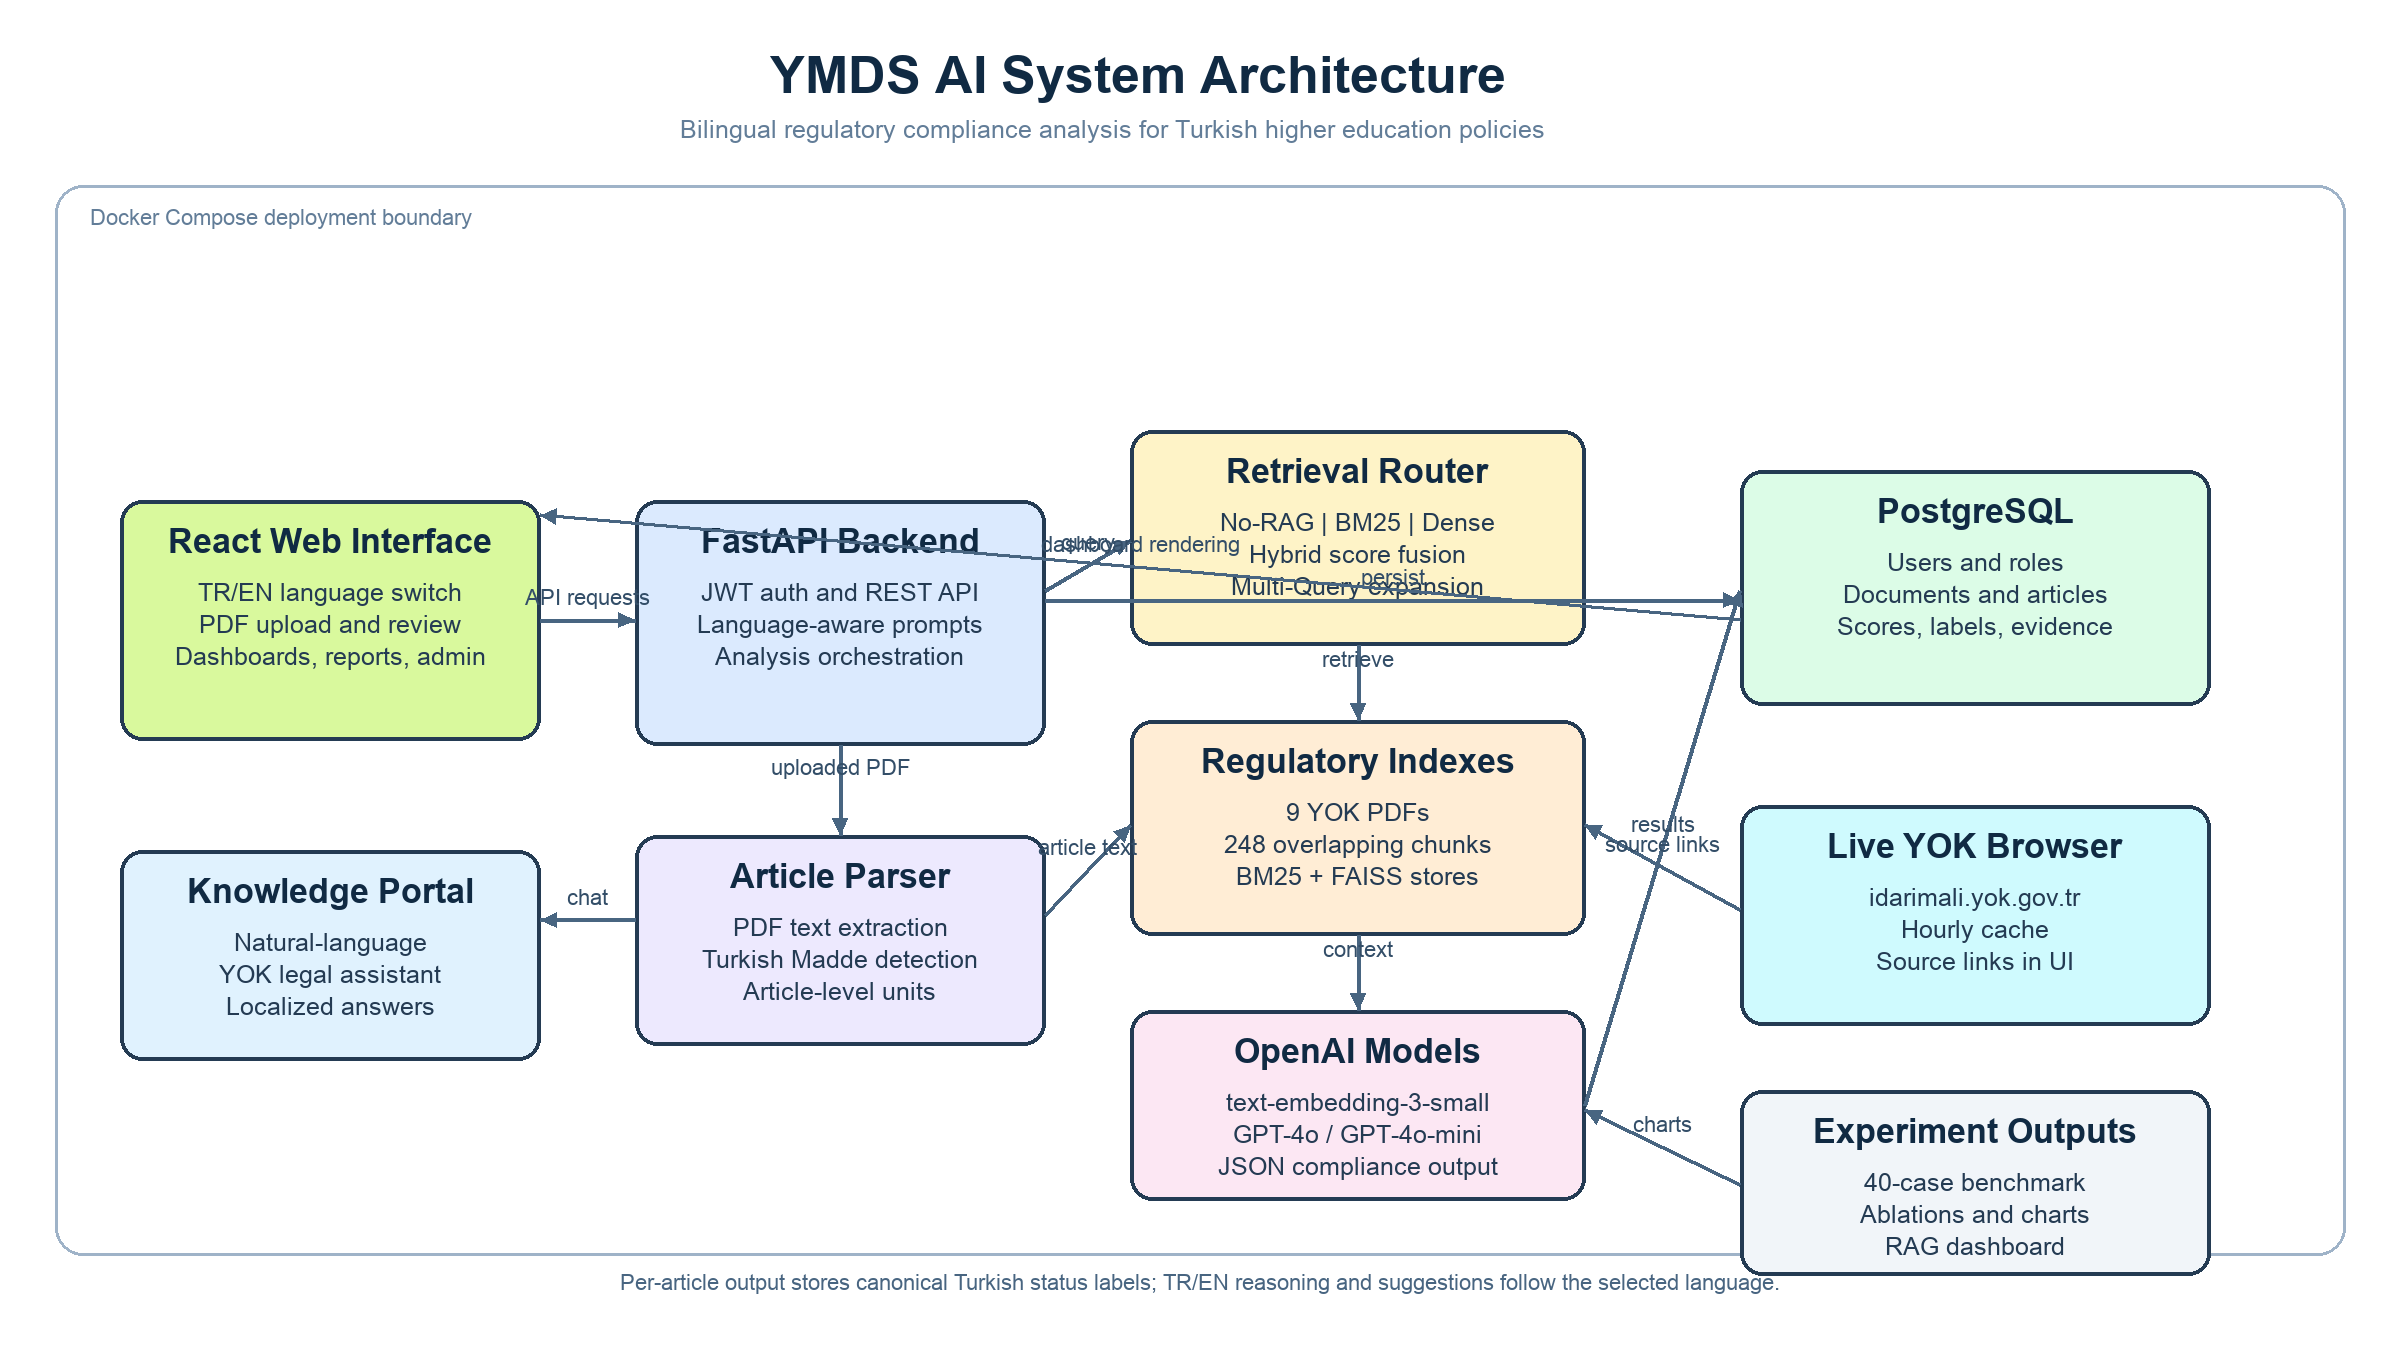
\includegraphics[width=0.92\textwidth]{figures/fig01_architecture.pdf}
  \includegraphics[width=0.92\textwidth]{figures/SystemDesign.png}
  \caption{Overview of the YMDS AI system architecture. University policy
    documents are uploaded via the React dashboard and forwarded to the FastAPI
    backend. The backend splits each document into articles, invokes the selected
    RAG pipeline to retrieve relevant YÖK regulation chunks from the knowledge
    base, and passes the retrieved context to the LLM for per-article compliance
    assessment. Results are stored in PostgreSQL and rendered in the dashboard
    with article-level status labels and a document-level compliance score.}
  \label{fig:architecture}
\end{figure*}

%% ════════════════════════════════════════════════════════════════════════════
%% SECTION 4 — METHODOLOGY
%% ════════════════════════════════════════════════════════════════════════════
\section{Methodology}
\label{sec:methodology}
This section describes the experimental methodology: how we built the evaluation dataset, how we run the benchmark, and how we measure performance.

\subsection{Benchmark Dataset Construction}

A core challenge in this work was constructing a test set that actually requires retrieval to answer correctly. If we created generic compliance questions about widely-known regulations, a language model could answer them from its training data alone — making it impossible to measure the contribution of the retrieval component. We therefore designed a \textit{RAG-aware} test set.

To build the dataset, we identified specific passages in the YÖK regulatory documents that contain concrete details: exact article numbers, numerical thresholds (e.g., minimum GPA requirements, maximum study durations), and procedural rules. For each selected passage, we generated a synthetic university procedure document that either correctly follows the regulation (compliant), partially follows it (partial), or clearly violates a specific numerical or procedural requirement (non-compliant). The violation in non-compliant cases was always a concrete change — for example, changing a required minimum score from 55 to 45, or shortening a mandated notice period.

Gold labels were assigned by running GPT-4o \textit{with the original YÖK passage as context} (i.e., oracle evaluation). This ensures that the gold label reflects the actual regulatory requirement rather than the model's general intuition. Cases where the oracle and the generated label disagreed were discarded.

The final dataset contains 40 cases: 13 compliant, 14 partial, and 13 non-compliant. Cases span nine source documents and cover diverse topic areas including graduate admission, GPA requirements, financial aid, international student rules, and minor program enrollment.

\subsection{Evaluation Pipelines}

We evaluate five retrieval pipeline configurations, each combined with two LLM backends (GPT-4o and GPT-4o-mini), for a total of ten system configurations. Each configuration is evaluated on all 40 test cases, giving 400 LLM calls in total for the main benchmark.

All pipelines use the same document collection and chunking parameters (350-word chunks, 59-word overlap, 248 total chunks). For retrieval pipelines, the default retrieval depth is Top-$K = 5$, which was identified as optimal in our ablation study (Section~\ref{sec:results}).

\subsection{Evaluation Metrics}

\paragraph{Classification Accuracy.} Our primary metric is exact-match accuracy: the fraction of test cases where the system's predicted label (compliant / partial / non-compliant) matches the gold label.

\paragraph{Per-Class Accuracy.} Because the task is a three-class classification problem, we also report per-class accuracy (recall per class) to detect label bias. This is important because, as we discuss in Section~\ref{sec:results}, all models show a strong preference for the \textit{partial} label.

\paragraph{Latency.} We measure mean wall-clock latency per request (seconds), including the API round-trip time.

\paragraph{Cost.} We compute the total API cost for evaluating all 40 cases per configuration, using OpenAI's published pricing (GPT-4o: \$2.50/1M input tokens, \$10.00/1M output tokens; GPT-4o-mini: \$0.15/1M input tokens, \$0.60/1M output tokens at time of writing).

\subsection{Ablation Studies}

We conduct two ablation studies using the BM25 pipeline with GPT-4o-mini, which is a cost-effective configuration that allows us to run many experiments without large API costs.

\paragraph{Chunk Size Ablation.} We vary the chunk size across four values: 150, 250, 350, and 500 words, while keeping all other parameters fixed (Top-$K = 5$, overlap = 17\% of chunk size). For each chunk size, we rebuild the BM25 index from scratch and evaluate on the full 40-case test set.

\paragraph{Top-K Ablation.} We fix the chunk size at 350 words and vary the retrieval depth $K \in \{1, 3, 5, 10\}$. This measures how sensitive performance is to the number of retrieved passages provided as context to the LLM.


%% ════════════════════════════════════════════════════════════════════════════
%% SECTION 5 — EXPERIMENTAL SETUP
%% ════════════════════════════════════════════════════════════════════════════
\section{Experimental Setup}
\label{sec:setup}
\subsection{Implementation Details}

ComplianceAI is implemented in Python 3.14. The backend uses FastAPI for the REST API layer, \texttt{rank\_bm25} for sparse retrieval, \texttt{faiss-cpu} for dense vector search, \texttt{pypdf} for PDF text extraction, and the OpenAI Python SDK for LLM calls. The frontend is built with React. All experiments were run on a MacBook Pro (Apple M-series CPU, 16 GB RAM). No GPU was used; all LLM inference was via the OpenAI API.

\subsection{Knowledge Base}

The regulatory knowledge base consists of nine PDF documents obtained from the YÖK website and Istanbul Bilgi University's official resources. After chunking (350 words, 59-word overlap), the corpus contains 248 chunks. The dense index uses OpenAI's \texttt{text-embedding-3-small} model with 384-dimensional projections, which was chosen for its strong multilingual performance and low cost relative to larger embedding models.

\subsection{LLM Configuration}

Both GPT-4o (\texttt{gpt-4o-2024-08-06}) and GPT-4o-mini (\texttt{gpt-4o-mini-2024-07-18}) were evaluated. Temperature was set to 0.0 for all evaluation calls to ensure reproducible outputs. The system prompt instructs the model to return a valid JSON object with four fields: compliance score (0--100), label, explanation, and a list of referenced articles. A response format constraint (\texttt{response\_format: \{type: "json\_object"\}}) was applied to prevent malformed outputs.

\subsection{Benchmark Dataset}

The RAG-aware test set (40 cases, 13/14/13 class split) was constructed as described in Section~\ref{sec:methodology}. Dataset generation cost approximately \$0.80 in API fees. All test cases, gold labels, and source passages are included in the accompanying repository.

\subsection{Reproducibility}

All experiments are fully reproducible using the provided scripts. The benchmark script (\texttt{run\_benchmark\_balanced.py}) accepts a seed argument and logs all LLM outputs to a CSV file. The ablation scripts (\texttt{ablation\_bm25\_fast.py}) similarly log all intermediate results.


%% ════════════════════════════════════════════════════════════════════════════
%% SECTION 6 — RESULTS AND DISCUSSION
%% ════════════════════════════════════════════════════════════════════════════
\section{Results and Discussion}
\label{sec:results}
How much does retrieval actually help? Our experiments give a clear answer.
Table~\ref{tab:main_results} shows the full results across all ten
configurations, and Figure~\ref{fig:accuracy} makes the pattern immediately
visible: every RAG pipeline beats the no-RAG baseline.

To put those numbers in context: a random guesser on our three-class problem
would score 33.3\%. No-RAG sits barely above that (37.5\%), which confirms
that our benchmark is genuinely hard --- the model cannot rely on memorized
knowledge to answer correctly.

\subsection{Main Benchmark Results}

\begin{table*}[t]
\centering
\footnotesize
\caption{Results on the 40-case RAG-aware benchmark (N=40, three classes).
  Accuracy = exact-match label accuracy. Cost = total API cost for all 40
  evaluations. Best accuracy highlighted in bold.}
\label{tab:main_results}
\setlength{\tabcolsep}{8pt}
\begin{tabular}{llrrrr}
\toprule
Pipeline      & Model        & Accuracy        & Mean Score & Latency (s) & Cost (USD) \\
\midrule
BM25          & GPT-4o       & \textbf{47.5\%} & 70.6       & 2.36        & 0.144 \\
BM25          & GPT-4o-mini  & 45.0\%          & 80.2       & 2.15        & \textbf{0.008} \\
Dense         & GPT-4o       & 32.5\%          & 68.1       & 1.99        & 0.146 \\
Dense         & GPT-4o-mini  & 45.0\%          & 77.2       & 2.32        & \textbf{0.008} \\
Hybrid        & GPT-4o       & \textbf{47.5\%} & 69.9       & 1.82        & 0.145 \\
Hybrid        & GPT-4o-mini  & \textbf{47.5\%} & 77.6       & 1.71        & \textbf{0.008} \\
Multi-Query   & GPT-4o       & 45.0\%          & 71.4       & 1.94        & 0.145 \\
Multi-Query   & GPT-4o-mini  & 42.5\%          & 80.0       & 2.18        & \textbf{0.008} \\
No-RAG        & GPT-4o       & 37.5\%          & 74.1       & 4.06        & 0.060 \\
No-RAG        & GPT-4o-mini  & 37.5\%          & 87.8       & 1.90        & 0.003 \\
\midrule
Random chance & ---          & 33.3\%          & ---        & ---         & --- \\
\bottomrule
\end{tabular}
\end{table*}

\paragraph{Which pipeline wins?}
Hybrid and BM25 are the clear winners at \textbf{47.5\%} --- a
\textbf{+10 percentage point gain} over no-RAG.
Dense retrieval is the surprise loser: Dense + GPT-4o scores only 32.5\%,
actually \textit{below} the no-RAG baseline.
We think BM25's exact-match scoring handles specialized Turkish legal
terminology better than vector similarity in this domain.
Multi-Query performs in the middle, suggesting that expanding the query
sometimes helps but can also pull in off-topic passages.

\paragraph{Does the bigger model help?}
Mostly no --- and that is actually good news for deployment.
As Figure~\ref{fig:model_comparison} shows, GPT-4o-mini matches or beats
GPT-4o in most configurations.
For Hybrid retrieval, both tie at 47.5\% while GPT-4o costs
\textbf{19$\times$ more} per query (\$0.145 vs.\ \$0.008 for 40 cases).
Figure~\ref{fig:cost} shows the full cost-performance trade-off:
GPT-4o-mini points consistently appear in the high-accuracy, low-cost region.

\subsection{Where Models Struggle: Per-Class Breakdown}

The overall accuracy numbers tell only part of the story.
Table~\ref{tab:perclass} breaks down recall by compliance class, and
Figure~\ref{fig:heatmap} visualizes this as a heatmap.

\begin{table}[H]
\centering
\footnotesize
\caption{Per-class recall for selected configurations.
  Compliant: 13 cases. Partial: 14 cases. Non-compliant: 13 cases.}
\label{tab:perclass}
\begin{tabular}{llrrr}
\toprule
Pipeline    & Model        & Comp. & Partial & Non-Comp. \\
\midrule
Hybrid      & GPT-4o       & 46\%  & 93\%    & 0\% \\
Hybrid      & GPT-4o-mini  & 54\%  & 71\%    & 15\% \\
BM25        & GPT-4o       & 46\%  & 93\%    & 0\% \\
BM25        & GPT-4o-mini  & 62\%  & 57\%    & 15\% \\
No-RAG      & GPT-4o       & 31\%  & 71\%    & 8\% \\
No-RAG      & GPT-4o-mini  & 69\%  & 43\%    & 0\% \\
\bottomrule
\end{tabular}
\end{table}

The pattern in Figure~\ref{fig:heatmap} is striking.
Models are excellent at spotting \textit{partial} compliance (up to 93\%),
but almost completely miss \textit{non-compliant} documents ---
GPT-4o in the Hybrid configuration scores \textbf{0\%} on non-compliant cases.
Every time a document clearly violates a regulation, the model defaults
to ``partial'' instead.

This is not a quirk of our system --- it reflects a well-known tendency of
large language models to hedge rather than make strong negative
judgments \citep{Fazlija2024, Deshpande2024}.
For anyone deploying ComplianceAI in practice, this matters:
the system is good at flagging documents that are \textit{not clearly okay},
but human reviewers should make the final call on anything flagged as
non-compliant. Figure~\ref{fig:score_dist} further illustrates this
by showing how predicted compliance scores distribute across all pipelines.

\subsection{How Much Context Is Enough? Chunk Size Ablation}

One of the most practical decisions in building a RAG system is how to
chunk the source documents.
Table~\ref{tab:chunk_ablation} and Figure~\ref{fig:chunk_ablation} show
what happens as we sweep chunk sizes from 150 to 500 words.

\begin{table}[H]
\centering
\footnotesize
\caption{Chunk size ablation (BM25, GPT-4o-mini, Top-$K{=}5$).}
\label{tab:chunk_ablation}
\begin{tabular}{lrr}
\toprule
Chunk Size (words) & Accuracy & Latency (s) \\
\midrule
150                & 47.5\%   & 2.26 \\
250                & 50.0\%   & 1.95 \\
\textbf{350}       & \textbf{52.5\%} & 2.13 \\
500                & 40.0\%   & 2.11 \\
\bottomrule
\end{tabular}
\end{table}

The result is a clear inverted-U curve: accuracy climbs from 150 to 350
words, then drops sharply at 500.
\textbf{350 words is optimal at 52.5\%} --- 12 percentage points above
the 500-word setting.
YÖK regulation articles typically span 200--400 words, so a 350-word chunk
captures one complete article most of the time.
At 500 words, two articles get bundled together and the model receives
mixed signals.

\subsection{How Deep to Retrieve? Top-K Ablation}

Table~\ref{tab:topk_ablation} and Figure~\ref{fig:topk_ablation} show
the effect of retrieval depth $K$.

\begin{table}[H]
\centering
\footnotesize
\caption{Top-$K$ ablation (BM25, GPT-4o-mini, chunk size = 350).}
\label{tab:topk_ablation}
\begin{tabular}{lrr}
\toprule
Top-$K$ & Accuracy & Latency (s) \\
\midrule
1       & 50.0\%   & 1.85 \\
3       & 50.0\%   & 1.95 \\
\textbf{5}  & \textbf{52.5\%} & 2.04 \\
10      & 50.0\%   & 2.07 \\
\bottomrule
\end{tabular}
\end{table}

$K{=}5$ is optimal at 52.5\%, while other values plateau at 50.0\%.
Five chunks are enough to cover most compliance questions, which typically
involve one or two regulation articles plus some surrounding context.
Beyond five, extra chunks add latency but not accuracy.

\subsection{Response Time in Practice}

Figure~\ref{fig:latency} summarizes mean latency across all configurations.
The fastest RAG option is \textbf{Hybrid + GPT-4o-mini at 1.71 seconds}
per request --- fast enough for interactive use.
No-RAG + GPT-4o is counterintuitively the \textit{slowest} (4.06 seconds),
because without retrieval the full document is included in the prompt,
making inputs much longer.

\subsection{Key Takeaways}

Our experiments lead to three practical recommendations:

\begin{enumerate}
  \item \textbf{Retrieve. Always.}
    Even simple BM25 adds 10 percentage points over no-RAG.
    Hybrid is the most reliable choice.

  \item \textbf{Use GPT-4o-mini.}
    It matches GPT-4o accuracy at 19$\times$ lower cost.
    For a compliance tool processing hundreds of documents per year,
    this is a deciding factor.

  \item \textbf{Keep humans in the loop for non-compliant verdicts.}
    Models systematically miss violations. Use ComplianceAI as a
    first-pass filter, not a final judge.
\end{enumerate}


%% ── Inline Figures (generated by generate_paper_figures.py) ──────────────

\begin{figure}[h]
  \centering
  
\includegraphics[width=\columnwidth]{figures/fig02_accuracy_bar.pdf}
  \caption{Classification accuracy (\%) by retrieval pipeline and LLM model.
    Hybrid and BM25 with either model achieve 47.5\%, while Dense + GPT-4o
    performs worst (32.5\%).}
  \label{fig:accuracy}
\end{figure}

\begin{figure}[h]
  \centering
  
\includegraphics[width=\columnwidth]{figures/fig03_perclass_heatmap.pdf}
  \caption{Per-class accuracy heatmap. Green indicates high recall, red indicates
    low recall. All models show near-zero recall for the non-compliant class.}
  \label{fig:heatmap}
\end{figure}

\begin{figure}[h]
  \centering
  
\includegraphics[width=\columnwidth]{figures/fig04_cost_performance.pdf}
  \caption{Cost--performance trade-off. GPT-4o-mini (circles) achieves
    equivalent or higher accuracy than GPT-4o (squares) at approximately
    19$\times$ lower API cost across all pipelines.}
  \label{fig:cost}
\end{figure}

\begin{figure}[h]
  \centering
  
\includegraphics[width=\columnwidth]{figures/fig05_chunk_ablation.pdf}
  \caption{Effect of chunk size on (a) classification accuracy and (b)
    latency. Accuracy peaks at 350 words and drops sharply at 500 words.
    BM25 pipeline, GPT-4o-mini, Top-$K{=}5$.}
  \label{fig:chunk_ablation}
\end{figure}

\begin{figure}[h]
  \centering
  
\includegraphics[width=\columnwidth]{figures/fig06_topk_ablation.pdf}
  \caption{Effect of retrieval depth Top-$K$ on (a) accuracy and (b)
    latency. $K{=}5$ achieves the highest accuracy (52.5\%).}
  \label{fig:topk_ablation}
\end{figure}

\begin{figure}[h]
  \centering
  
\includegraphics[width=\columnwidth]{figures/fig07_score_distribution.pdf}
  \caption{Distribution of predicted compliance scores (0--100) by retrieval
    pipeline. Dashed lines indicate the compliant ($\geq 70$) and
    non-compliant ($< 30$) thresholds.}
  \label{fig:score_dist}
\end{figure}

\begin{figure}[h]
  \centering
  
\includegraphics[width=\columnwidth]{figures/fig08_latency.pdf}
  \caption{Mean response latency per request. Hybrid + GPT-4o-mini is
    the fastest RAG configuration (1.71\,s mean). No-RAG + GPT-4o is
    the slowest (4.06\,s) due to longer input prompts.}
  \label{fig:latency}
\end{figure}

\begin{figure}[h]
  \centering
  
\includegraphics[width=\columnwidth]{figures/fig09_model_comparison.pdf}
  \caption{GPT-4o vs.~GPT-4o-mini accuracy per pipeline, with
    $\Delta$ values indicating the GPT-4o advantage. GPT-4o-mini
    is competitive or superior in most configurations.}
  \label{fig:model_comparison}
\end{figure}

%% ════════════════════════════════════════════════════════════════════════════
%% SECTION 7 — CONCLUSION
%% ════════════════════════════════════════════════════════════════════════════
\section{Conclusion}
\label{sec:conclusion}
We presented ComplianceAI, a retrieval-augmented generation system for
automatically checking whether university policy documents comply with YÖK
regulations. The system was motivated by a genuine administrative need:
compliance review at Turkish universities is a manual, time-consuming process
that requires reading through dense legal text.
We built something that can meaningfully assist administrative staff ---
not replace them, but make their work faster and more targeted.

\subsection{Summary of Findings}

Our evaluation on a 40-case RAG-aware benchmark produced clear,
reproducible findings.
Retrieval helps: the best RAG configurations reach \textbf{47.5\% accuracy}
compared to \textbf{37.5\% for no-RAG}, a 10 percentage point improvement
on a benchmark specifically designed to require regulatory knowledge
(see Table~\ref{tab:main_results} and Figure~\ref{fig:accuracy}).
Sparse and hybrid retrieval outperform dense-only retrieval in this domain,
likely because BM25's exact-match scoring handles Turkish legal terminology
well without relying on embedding quality.
GPT-4o-mini matches GPT-4o performance at 19$\times$ lower cost ---
a significant practical advantage for a system meant to run continuously
in a university environment.
Optimal hyperparameters are 350-word chunks and Top-5 retrieval depth,
as confirmed by the ablation studies in
Tables~\ref{tab:chunk_ablation} and \ref{tab:topk_ablation} and
Figures~\ref{fig:chunk_ablation} and \ref{fig:topk_ablation}.

The most important limitation is that all models systematically fail to
detect non-compliant documents, defaulting to ``partial'' even for clear
violations (Table~\ref{tab:perclass}, Figure~\ref{fig:heatmap}).
This means the system is currently best positioned as a \textit{risk filter}
that flags documents for human review, not as a standalone compliance auditor.

\subsection{Limitations}

\textbf{Benchmark size.}
Our test set contains 40 cases. While this is sufficient to observe
consistent trends, a larger annotated dataset --- ideally with human expert
labels rather than LLM-generated gold labels --- would give more reliable
performance estimates.

\textbf{Single institution.}
We built and evaluated the system using Istanbul Bilgi University documents.
Whether the findings generalize across institutions with different policy
styles and document formats is an open question.

\textbf{Manual document management.}
The current knowledge base requires manual updates whenever YÖK revises
a regulation. This is manageable for a prototype but not scalable
for a production system used across many institutions.

\textbf{Non-compliant detection.}
Models consistently under-predict the non-compliant class.
This is a fundamental behavior of current LLMs, not a hyperparameter problem,
and will likely require fine-tuning or a different problem formulation to fix.

\subsection{Future Work}

Several directions are worth pursuing.

\paragraph{Live regulatory updates.}
The most immediate improvement would be to automate regulatory document
updates by integrating directly with the YÖK web portal.
When YÖK publishes a new or revised regulation, the system would
automatically fetch the document, chunk it, update the indexes, and notify
administrators. This would eliminate the current manual maintenance step
and ensure the system always operates on up-to-date regulations.

\paragraph{Broader deployment.}
Although ComplianceAI was built for Istanbul Bilgi University, it is designed
to be institution-agnostic. Any Turkish university could deploy the same system
by loading their own institutional documents alongside the shared YÖK knowledge
base. Beyond Turkey, the same approach is directly applicable to other
higher education regulatory systems --- ECTS credit regulations in Europe,
ABET accreditation requirements in the United States, or country-specific
higher education laws elsewhere.

\paragraph{Better non-compliant detection.}
Fine-tuning a smaller language model on compliance-specific examples, or
using adversarial training with deliberately non-compliant document pairs,
could improve recall for the non-compliant class.

\paragraph{Graph-based retrieval.}
YÖK regulations frequently cross-reference each other.
Graph-based retrieval approaches, as explored by \citet{Masoudifard2024},
could better capture these relationships and improve performance on
multi-article compliance questions.

\paragraph{Human annotation.}
Constructing a human-annotated benchmark with cases drawn from real
administrative documents would significantly strengthen evaluation reliability
and provide a community resource for future work in this area.

\subsection{Closing Remarks}

ComplianceAI demonstrates that retrieval-augmented generation is a practical
and effective approach for regulatory compliance checking in a specialized
legal domain. The system is not yet production-ready as a standalone tool,
but it meaningfully accelerates the compliance review process by surfacing
relevant regulation passages and providing an initial classification.
We hope the open-source code, benchmark dataset, and evaluation methodology
we provide will serve as a foundation for future work --- whether at Turkish
universities seeking to modernize their administrative processes,
or in other regulatory domains where the same challenges apply.


%% ════════════════════════════════════════════════════════════════════════════
%% CRediT Author Contribution Statement
%% ════════════════════════════════════════════════════════════════════════════
\printcredits

%% ════════════════════════════════════════════════════════════════════════════
%% Declaration of Competing Interest
%% ════════════════════════════════════════════════════════════════════════════
\section*{Declaration of Competing Interest}
The authors declare that they have no known competing financial interests or
personal relationships that could have appeared to influence the work reported
in this paper.

%% ════════════════════════════════════════════════════════════════════════════
%% Acknowledgements
%% ════════════════════════════════════════════════════════════════════════════
\section*{Acknowledgements}
This work was conducted as part of the Senior Design Project at Istanbul Bilgi
University, Department of Computer Engineering. The authors thank the
Department of Student Affairs for providing access to institutional policy
documents used in the evaluation.

%% ════════════════════════════════════════════════════════════════════════════
%% Data Availability
%% ════════════════════════════════════════════════════════════════════════════
\section*{Data Availability}
The benchmark test set, evaluation scripts, and FAISS index caches are
available at: \url{https://github.com/Asyaberk/YMDSAI}.
The YÖK regulatory documents used as the knowledge base are publicly available
at \url{https://www.yok.gov.tr}.

%% ════════════════════════════════════════════════════════════════════════════
%% Bibliography
%% ════════════════════════════════════════════════════════════════════════════
\bibliographystyle{cas-model2-names}
\bibliography{compliance_ai}

%% ════════════════════════════════════════════════════════════════════════════
%% APPENDIX A — System Prompt
%% ════════════════════════════════════════════════════════════════════════════
\appendix
\section{LLM System Prompt}
\label{app:prompt}

The following system prompt is used for all per-article LLM compliance reasoning calls
(reproduced verbatim from \texttt{backend/services/rag\_service.py}, \texttt{ARTICLE\_SYSTEM}):

\begin{verbatim}
Sen Türk yükseköğretim hukuku uzmanı bir denetçisin.
Sana incelenen bir üniversite yönetmeliğinin TEK BİR MADDESİ
ve referans YÖK mevzuat parçaları verilecek.

TEMEL İLKE: Uyumluluk = kelime kelime aynı olmak DEĞİL,
YÖK'ün düzenlediği amacı/hükmü karşılamak demektir.

UYUMLULUK TANIMLARI (4 seçenek):
- Uyumlu: Madde, YÖK'ün düzenlediği konuyu karşılıyor.
  İfade farklı olsa da aynı amacı güdüyor.
- Kısmen Uyumlu: Madde genel olarak doğru yönde ama
  (a) YÖK'ün zorunlu kıldığı spesifik bir unsur eksik, veya
  (b) belirsiz/muğlak ifadeler YÖK'ün net hükmünü tam
  karşılamıyor. Sağlanan YÖK parçaları bu maddeyle
  yalnızca dolaylı ilgiliyse de Kısmen Uyumlu ver.
- Uyumsuz: Aşağıdaki somut durumlardan biri varsa:
  (a) YÖK'ün belirlediği sayısal eşik/süre/oran farklıysa;
  (b) YÖK'ün zorunlu kıldığı onay makamı/prosedür yoksa;
  (c) YÖK'ün yasakladığı bir uygulama belgede varsa;
  (d) YÖK'ün tanımladığı hak/koruma belgede kısıtlanmışsa.
- Kapsam Dışı: YALNIZCA şu iki durumda kullan:
  (1) Bu konu YÖK mevzuatının hiçbir bölümünde düzenlenmemiş;
      üniversitenin tamamen serbest bırakıldığı idari konudur.
  (2) Madde yalnızca geçici/geçiş hükmü içeriyor.
  ÖNEMLI: Konu şunlardan biriyse Kapsam Dışı VERMEK YASAKTIR:
  Sınav, not sistemi, GANO/YANO/AGNO, ders kaydı, kayıt
  dondurma, mezuniyet, burs, disiplin, akademik takvim,
  ders programı, kredi sistemi, öğrenci kabulü.

ÇIKTI — yalnızca bu JSON (başka metin ekleme):
{
  "status": "<Uyumlu|Kısmen Uyumlu|Uyumsuz|Kapsam Dışı>",
  "similarity": <0.0–1.0, anlam örtüşmesi>,
  "yok_reference": "<ilgili YÖK mevzuat adı ve maddesi>",
  "yok_text": "<sağlanan YÖK parçalarından doğrudan alıntı>",
  "reasoning": [
    "<neden bu status: belgede ne diyor, YÖK ne diyor>",
    "<varsa eksiklik veya çelişki>"
  ],
  "suggestion": "<YALNIZCA Kısmen Uyumlu/Uyumsuz ise:
                  ne değiştirilmeli/eklenmeli? Uyumlu ise: ''>"
}
\end{verbatim}

%% ════════════════════════════════════════════════════════════════════════════
%% APPENDIX B — Application Screenshots
%% ════════════════════════════════════════════════════════════════════════════
\section{Application Screenshots}
\label{app:screenshots}

The following figures show the main pages of the deployed YMDS AI
web application. All screenshots are taken from the production deployment
running on \texttt{localhost} with Docker Compose
(FastAPI backend + React frontend + PostgreSQL).
The full source code is available at \url{https://github.com/Asyaberk/YMDSAI}.

\begin{figure}[H]
  \centering
  \fbox{\parbox{0.88\columnwidth}{\centering\vspace{2cm}
    \textit{[Placeholder — Compliance Analysis page:\newline
    document list with compliance scores and status badges]}
    \vspace{2cm}}}
  \caption{Compliance Analysis page. Uploaded documents are listed with
    their overall compliance score (0--100), status badge, and article
    breakdown counts.}
  \label{fig:app_analysis_list}
\end{figure}

\begin{figure}[H]
  \centering
  \fbox{\parbox{0.88\columnwidth}{\centering\vspace{2cm}
    \textit{[Placeholder — Article detail view:\newline
    per-article status, YÖK reference, similarity score, and suggestions]}
    \vspace{2cm}}}
  \caption{Article-level detail view. Each article is classified as
    Compliant, Partially Compliant, Out-of-Scope, or Non-Compliant, with
    the retrieved YÖK regulation text, similarity score, and
    an improvement suggestion.}
  \label{fig:app_article_detail}
\end{figure}

\begin{figure}[H]
  \centering
  \fbox{\parbox{0.88\columnwidth}{\centering\vspace{2cm}
    \textit{[Placeholder — Admin Dashboard:\newline
    document management table with PDF viewer and user statistics]}
    \vspace{2cm}}}
  \caption{Admin Dashboard. Administrators can view all uploaded documents
    across all users, open the original PDF, inspect per-document article
    statistics, and delete records.}
  \label{fig:app_admin}
\end{figure}

\begin{figure}[H]
  \centering
  \fbox{\parbox{0.88\columnwidth}{\centering\vspace{2cm}
    \textit{[Placeholder — RAG Experiments page:\newline
    pipeline comparison charts, ablation results, and per-class heatmap]}
    \vspace{2cm}}}
  \caption{RAG Experiments page. All benchmark results (accuracy, latency,
    cost) and ablation study charts are rendered from the live
    experimental outputs stored in the repository.}
  \label{fig:app_experiments}
\end{figure}

%% ════════════════════════════════════════════════════════════════════════════
%% APPENDIX C — Core Algorithms
%% ════════════════════════════════════════════════════════════════════════════
\section{Core Algorithms}
\label{app:algorithms}

This appendix provides formal pseudocode for two implementation-specific
components: the Turkish article boundary detector (Algorithm~\ref{alg:splitter}),
which is domain-novel, and the hybrid retrieval pipeline
(Algorithm~\ref{alg:hybrid}), whose linear score interpolation is detailed
here to distinguish it from a rank-position-based fusion approach.

\begin{algorithm}[htbp]
\DontPrintSemicolon
\SetKwInOut{Input}{Input}
\SetKwInOut{Output}{Output}
\caption{Turkish Article Boundary Detection}
\label{alg:splitter}

\Input{Raw PDF text $T$ (continuous string after \texttt{pypdf} extraction)}
\Output{List of articles $\mathcal{A} = [\{\text{number},\,\text{title},\,\text{text}\}]$}

$P_1 \leftarrow$ \texttt{(Madde|MADDE)\textbackslash s+(\textbackslash d+)\textbackslash s*[-\textendash\textemdash]} \tcp*{dash after number}
$P_2 \leftarrow$ \texttt{(Madde|MADDE)\textbackslash s*[-\textendash\textemdash]\textbackslash s*(\textbackslash d+)} \tcp*{dash before number}
$P_3 \leftarrow$ \texttt{(Madde|MADDE)\textbackslash s+(\textbackslash d+)\textbackslash s*\textbackslash(} \tcp*{parenthesis format}

$M \leftarrow \text{findall}(P_1, T)$\;
\lIf{$|M| < 2$}{ $M' \leftarrow \text{findall}(P_2, T)$;\quad \lIf{$|M'| > |M|$}{$M \leftarrow M'$} }
\lIf{$|M| < 2$}{ $M'' \leftarrow \text{findall}(P_3, T)$;\quad \lIf{$|M''| > |M|$}{$M \leftarrow M''$; \texttt{use\_paren} $\leftarrow$ True} }
\lIf{$|M| < 2$}{ \Return 500-word chunks of $T$ labelled B\"ol\"um 1, 2,\,\ldots }

\ForEach{$(i,\; m_i) \in \text{enumerate}(M)$}{
  art\_start $\leftarrow m_i.\text{start}()$\;
  art\_end $\leftarrow m_{i+1}.\text{start}()$ \textbf{if} $i+1 < |M|$ \textbf{else} $|T|$\;
  body $\leftarrow T[\text{art\_start}:\text{art\_end}]$, stripped of trailing page number\;
  \uIf{\texttt{use\_paren}}{
    title $\leftarrow$ content inside first \texttt{(\ldots)} following $m_i$\;
  }\Else{
    title $\leftarrow$ last 1--6 words preceding $m_i$ in current article span\;
  }
  append $\{\text{number}: \texttt{Madde}~i,\; \text{title},\; \text{text}: \text{body}\}$ to $\mathcal{A}$\;
}
\Return $\mathcal{A}$
\end{algorithm}

\bigskip

\begin{algorithm}[htbp]
\DontPrintSemicolon
\SetKwInOut{Input}{Input}
\SetKwInOut{Output}{Output}
\caption{Hybrid Retrieval via Linear Score Interpolation}
\label{alg:hybrid}

\Input{Query $q$; BM25 index $\mathcal{B}$; FAISS index $\mathcal{F}$; depth $K$; weight $\alpha = 0.5$}
\Output{Top-$K$ chunks ranked by hybrid score}

$R_B \leftarrow \text{BM25\_retrieve}(\mathcal{B}, q, 2K)$ \tcp*{sparse candidates with raw BM25 scores}
$R_F \leftarrow \text{FAISS\_retrieve}(\mathcal{F}, q, 2K)$ \tcp*{dense candidates with cosine scores}

\tcp{Min-max normalise each score list independently to $[0,1]$}
$\hat{s}_B[c] \leftarrow \dfrac{s_B[c] - \min_B}{\max_B - \min_B}$ \quad for each $c \in R_B$\;
$\hat{s}_F[c] \leftarrow \dfrac{s_F[c] - \min_F}{\max_F - \min_F}$ \quad for each $c \in R_F$\;

$S \leftarrow \{\}$\;
\ForEach{$c \in R_B$}{ $S[c] \mathrel{+}= (1-\alpha)\,\hat{s}_B[c]$ }
\ForEach{$c \in R_F$}{ $S[c] \mathrel{+}= \alpha\,\hat{s}_F[c]$ }

\Return top-$K$ chunks from $S$ sorted by score descending
\end{algorithm}

\smallskip
\noindent\textbf{Note on Multi-Query.} The Multi-Query pipeline generates two
additional query phrasings via an LLM call (temperature~$= 0.7$), runs
BM25 independently for each of the three queries (original plus two variants),
and merges results by union before re-ranking by BM25 score (Algorithm
line~2 of the BM25 path). This adds exactly one extra API call per request
and requires no additional index structures.

\end{document}
